\section{Results}\label{Sec:Results}

In this section, we describe the descriptive analysis of representative points in relation to the confidence regions, as well as revisiting hypotheses of white noise present in the literature.
Empirical experiments on the behavior of an emblematic sample when injecting correlation structures are also presented.

We employed the following factors in this study:
\begin{itemize}
\item Time series length $T\in\mathcal T=\{10^3, \num[scientific-notation=true]{5 e4}\}$,
\item Embedding dimension $D\in\mathcal D=\{3, 4, 5, 6\}$,and
\item Exponent of the $f^{-k}$ noise $k\in\mathcal K=\{0, 0.05, 0.1, 0.15, 0.2, 0.25, 0.3, 0.5, 1,\\ 1.5, 2, 2.5, 3\}$.
\item Time delay $\tau=\{1,10,30,50\}$.
\end{itemize}
%There were no significant differences in data in repeated experiments with time delays $\tau=\{1,10,30,50\}$. 
%Therefore, we obtained $1000$ independent series for each point in the factors set $\mathcal T\times \mathcal D\times \mathcal K$.

The data generation and analyses were performed using the \texttt R platform \cite{Rmanual} v.~3.6.3.
We used the \texttt{ggplot2} library \cite{ggplot2Wickman} for generating the plots.

\subsection{Descriptive analysis of representative data}

For the construction of the confidence regions presented in this work we use:
\begin{itemize}
    \item An set of $104596$ points in the $H \times C$ plane, referring to sequences of length $T = 1000$, for each combination of the factors $\mathcal T \times \mathcal D \times \mathcal{\tau}$, and
    \item  An another set of $2093$ points in the $H \times C$ plane, referring to sequences of length $T = 50000$, for each combination of factors $\mathcal T \times \mathcal D \times \mathcal{\tau}$.
\end{itemize}
Since the results involving the variation of the time delay parameter did not show a significant difference in repeated experiments, we don't consider it as a determinating factor during the execution of the algorithm.
On the other hand, we consider two determining variables during the generation of such sub-spaces: the embedding dimension and the length of the sequence.

\begin{figure}[H]
    \centering
    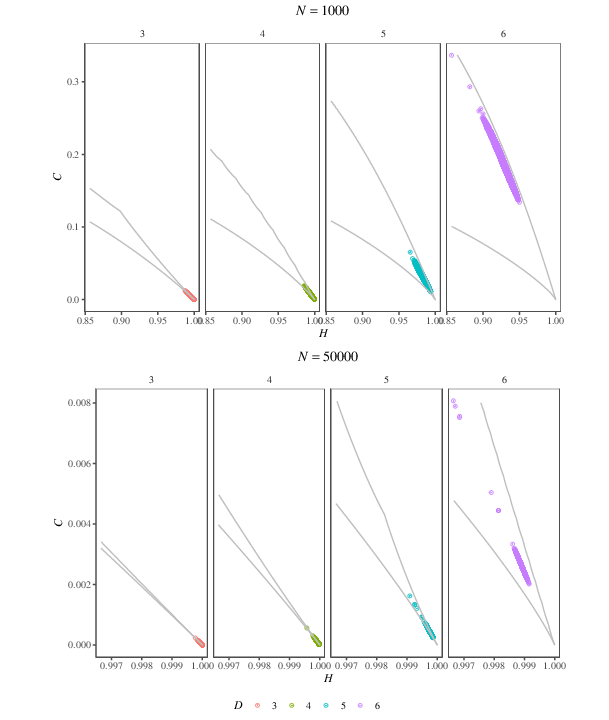
\includegraphics[width=\linewidth]{Figures/Points-PDF.png}
    \caption{White noise samples considered during the construction of the proposed confidence regions.}
    \label{fig:white-noise}
\end{figure}

In Fig.~\ref{fig:HC-PCA} we show the results obtained for $T = 50000$ in the scenarios of $D = 3$ and $D = 6$ in the new space defined by the PCA, together with the quantiles of $90\%$, $95\%$, $99\%$ and $99.9\%$.
We also show the projection of the $H \times C$ plane limits in this new representation space, as well as identifying the median of each data set, the latter being represented as the red dots present in the graphs.

\begin{figure}[H]
	\centering
	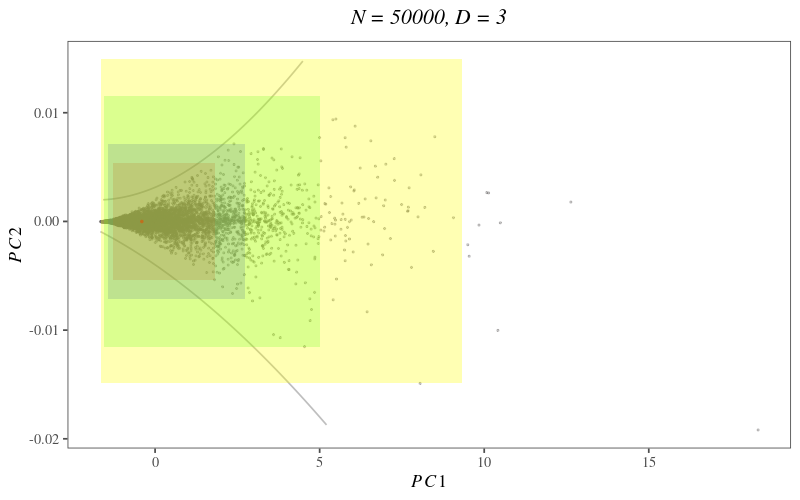
\includegraphics[width=.45\linewidth]{Figures/HC-PCA-Trozos-D3N50k.png}
	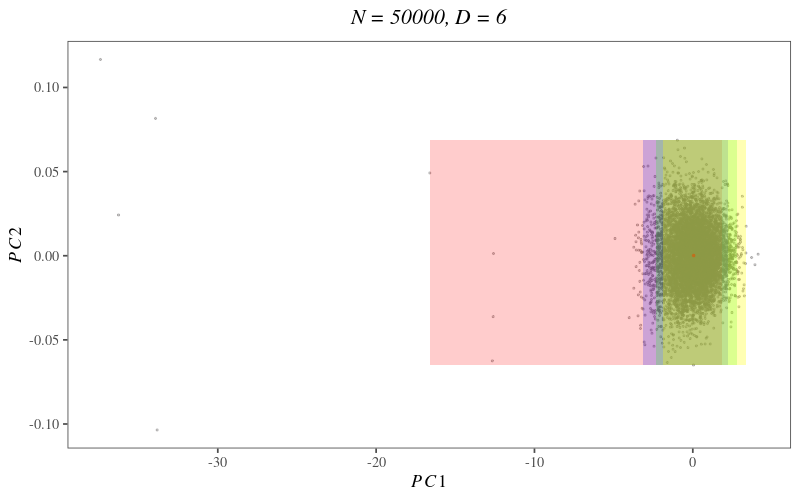
\includegraphics[width=.45\linewidth]{Figures/HC-PCA-Trozos-D6N50k.png}
	\caption{}
	\label{fig:HC-PCA}
\end{figure} 

As we can see in Fig.~\ref{fig:PCA-Hist} in the new representation space produced by the PCA, the data are not evenly distributed among the axes of the first main component, maintaining the character presented in the $H \times C$ plane, since such points tend to be concentrated close to the point $(1, 0)$.

\begin{figure}[H]
    \centering
    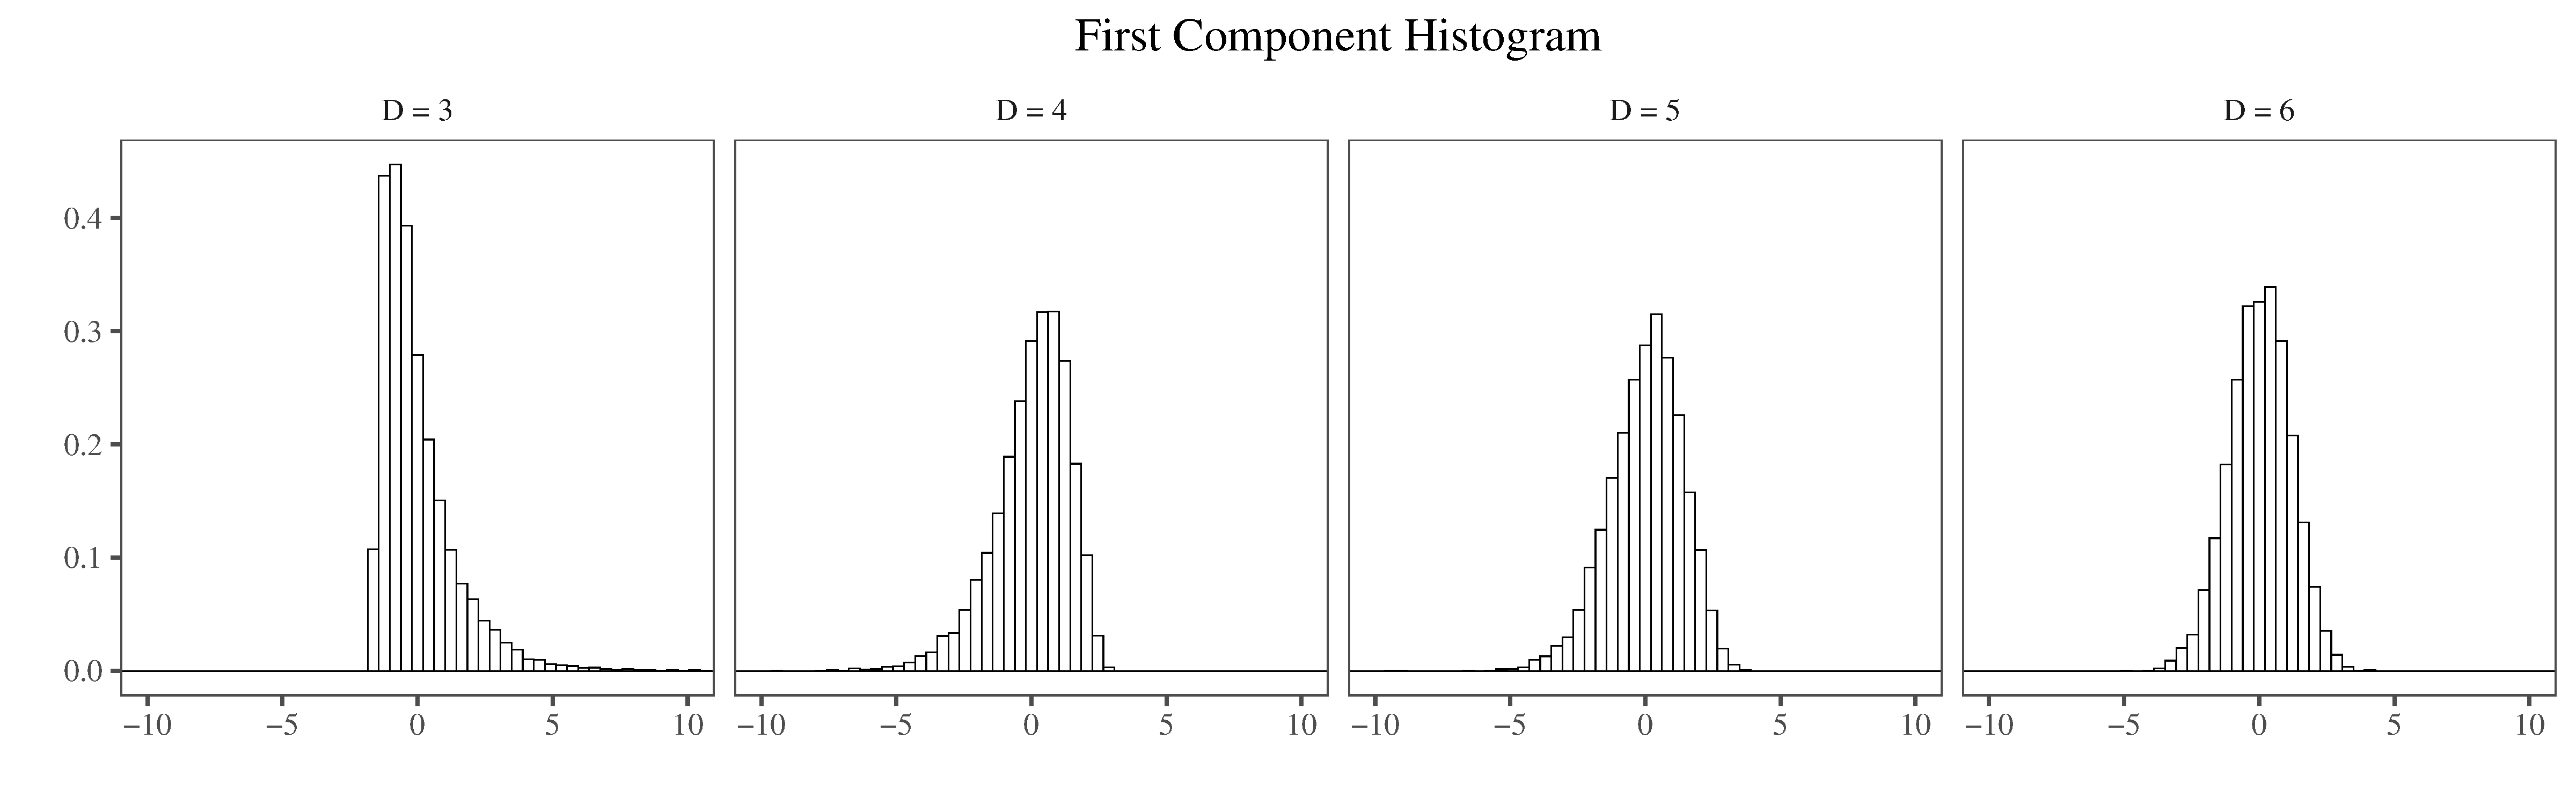
\includegraphics[width=\linewidth]{PCA-hist-50k}
    \caption{Histogram of the PCA first component }
    \label{fig:PCA-Hist}
\end{figure}

%\textcolor{red}{An\'alise descritiva: alguns pontos de $\Theta$ representativos:} 
\subsection{Testing White Noise in the confidence regions}

To test the efficiency of the confidence region calculated, we tested its applicability on a set of truly random data generated physically not used by the algorithm during its construction. 
The results can be seen in Fig.~\ref{fig:RNG}.

For small series, $N = 1000$, and $D = 3$ we managed to maintain exactly $99\%$ of the data in the confidence region of the same value, and as the dimension increased reach $96\%$ of the points.
On the other hand, there was a very large loss of points located in the region with $95\%$ confidence as the dimension increased.
A reasonable explanation for this event is given in the choice of the parameter itself.
It is known by definition that $D! << N$, which does not happen for such a sample size, thus presenting many missing patterns that lead to an unrepresentative probability distribution.
For larger series, $N = 50000$, although we observed a small drop in the percentage of data present in the region with $99\%$ confidence, there was a significant increase in points in the region with $95\%$ confidence, showing between $90\%$ and $88\%$ of the points when we vary the embedding dimension.

\begin{table}[H]
	\centering
	\caption{Results found it for samples of true random numbers}
	\label{tab:result1}
	\begin{tabular}{c*{3}rr}
		\toprule
		Algorithm & \multicolumn{1}{c}{$N$} & \multicolumn{1}{c}{$D$} & \multicolumn{1}{c}{\SI{95}{\percent}} & \multicolumn{1}{c}{\SI{99}{\percent}}\\
		\cmidrule(lr){1-1}
		\cmidrule(lr){2-2}
		\cmidrule(lr){3-3}
		\cmidrule(lr){4-4}
		\cmidrule(lr){5-5}
		True-Random & 1000 & 3 & $0.98$ & $1$\\
		&  & 4 & $0.98$ & $0.96$\\
		&  & 5 & $1$ & $0.94$\\
		&  & 6 & $0.97$ & $0.87$\\
		\cmidrule(lr){1-5}
		True-Random & 50000 & 3 & $0.97$ & $0.96$\\
		&  & 4 & $0.94$ & $0.95$\\
		&  & 5 & $0.97$ & $0.96$\\
		&  & 6 & $0.98$ & $0.99$\\
		\bottomrule
	\end{tabular}
\end{table}

\begin{figure}[H]
    \centering
    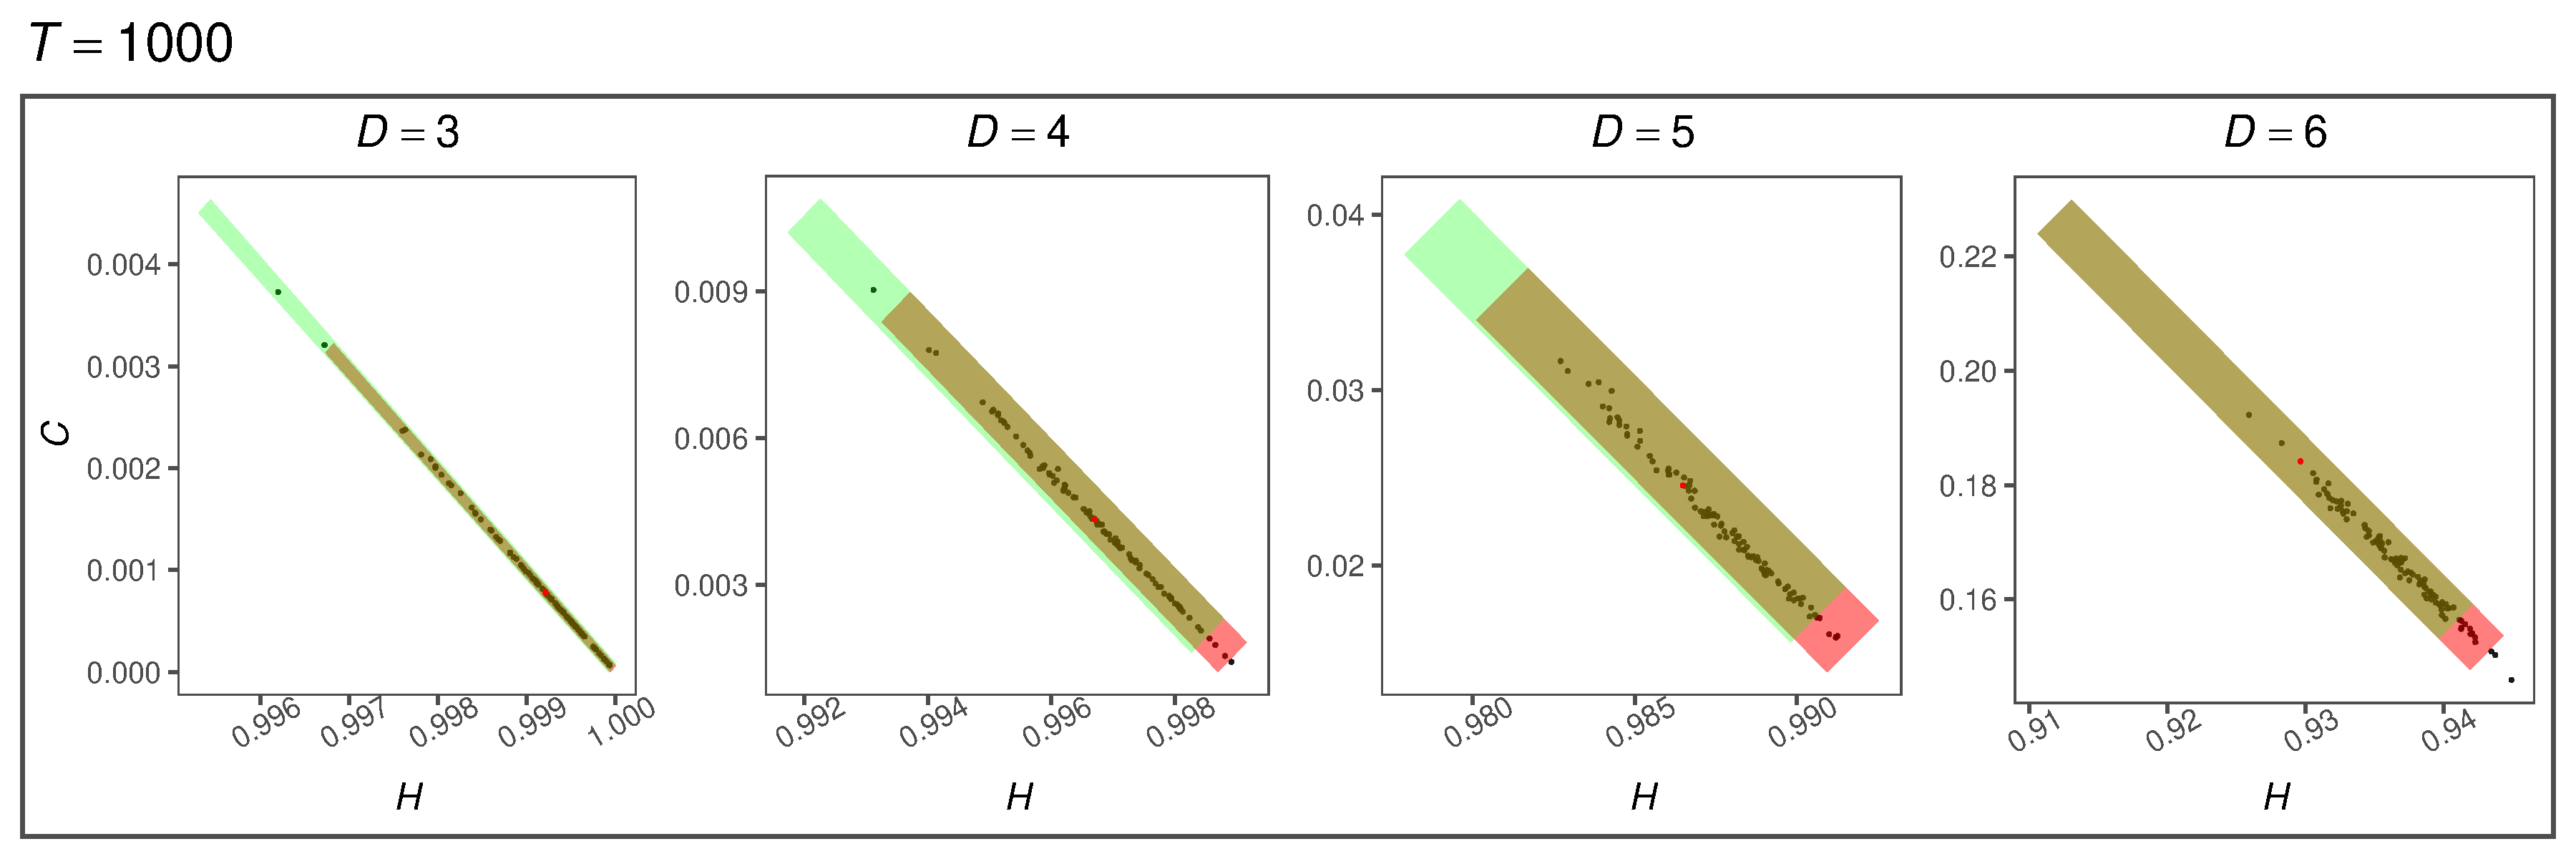
\includegraphics[width=\linewidth]{Figures/RNG-1000.pdf}
    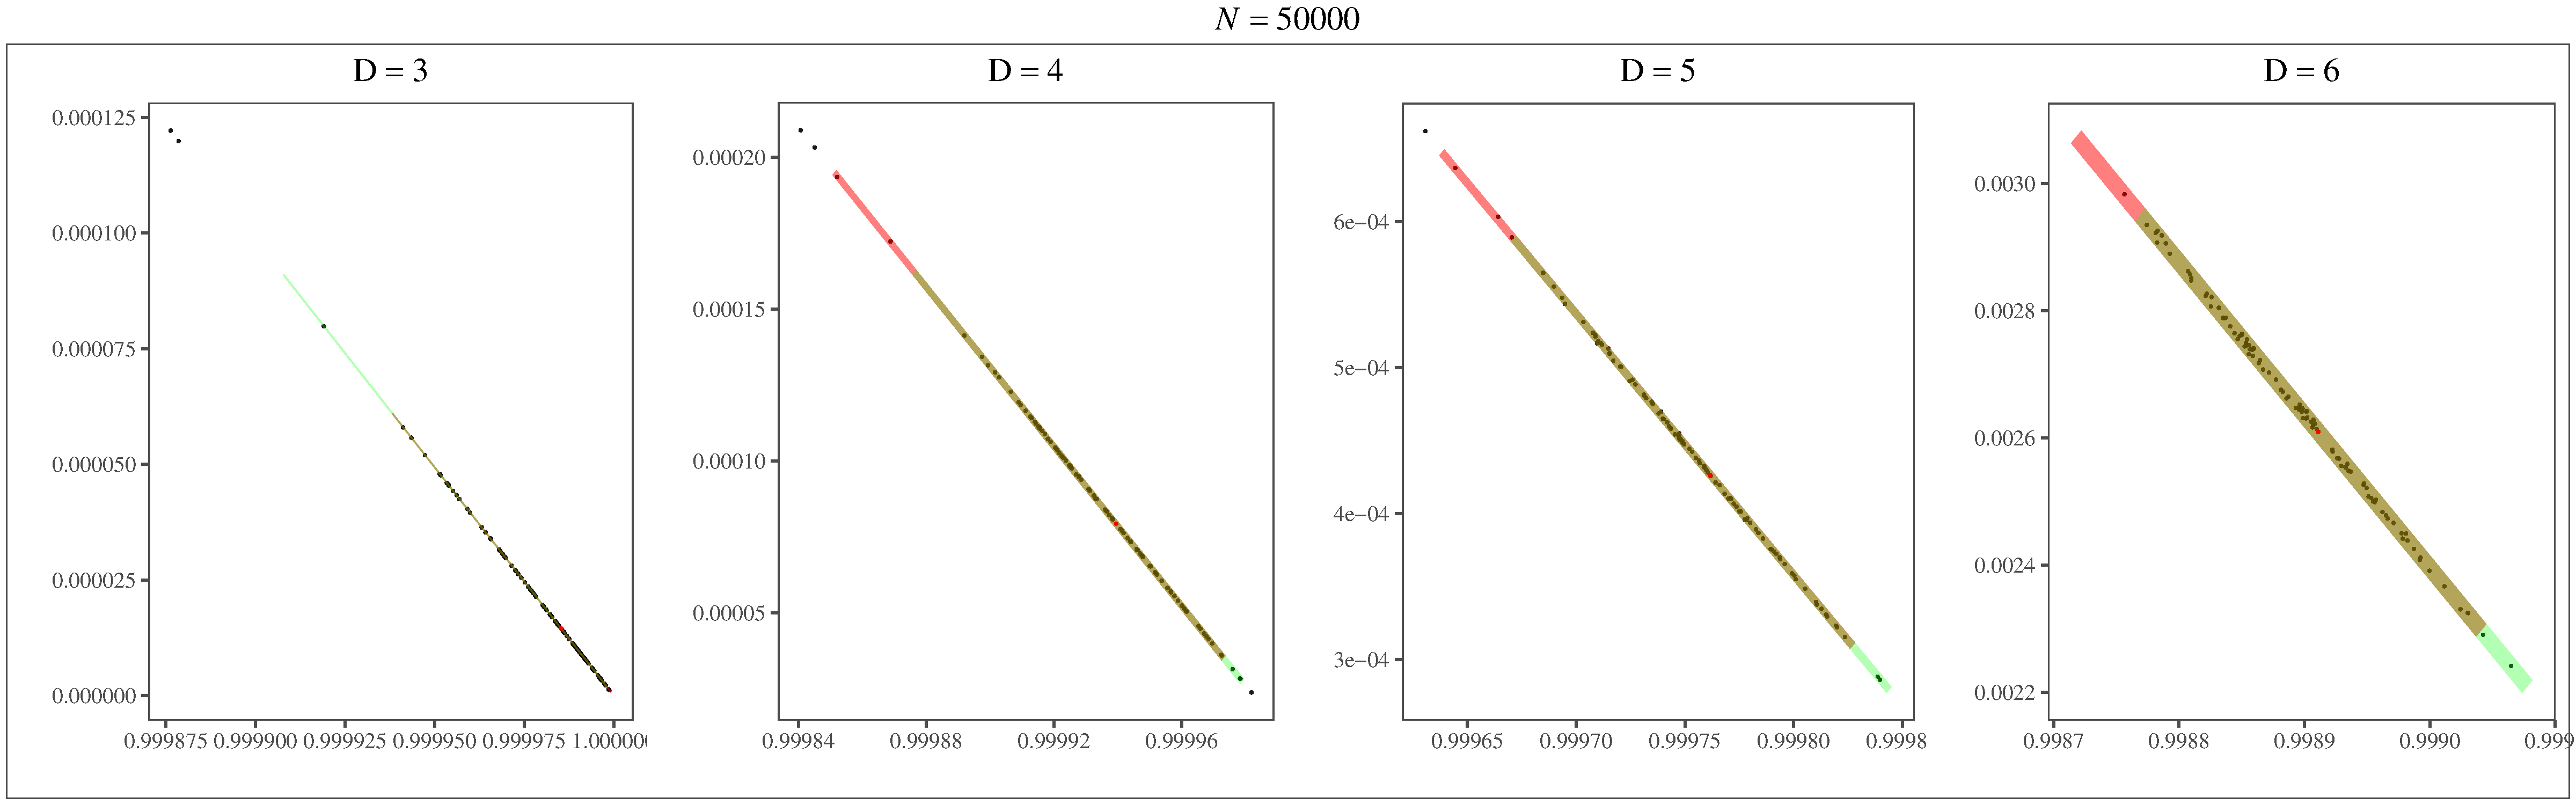
\includegraphics[width=\linewidth]{Figures/RNG-50000.pdf}
    \caption{White Noise in HC Plane}
    \label{fig:RNG}
\end{figure}

\begin{comment}
\begin{figure}[H]
    \centering
    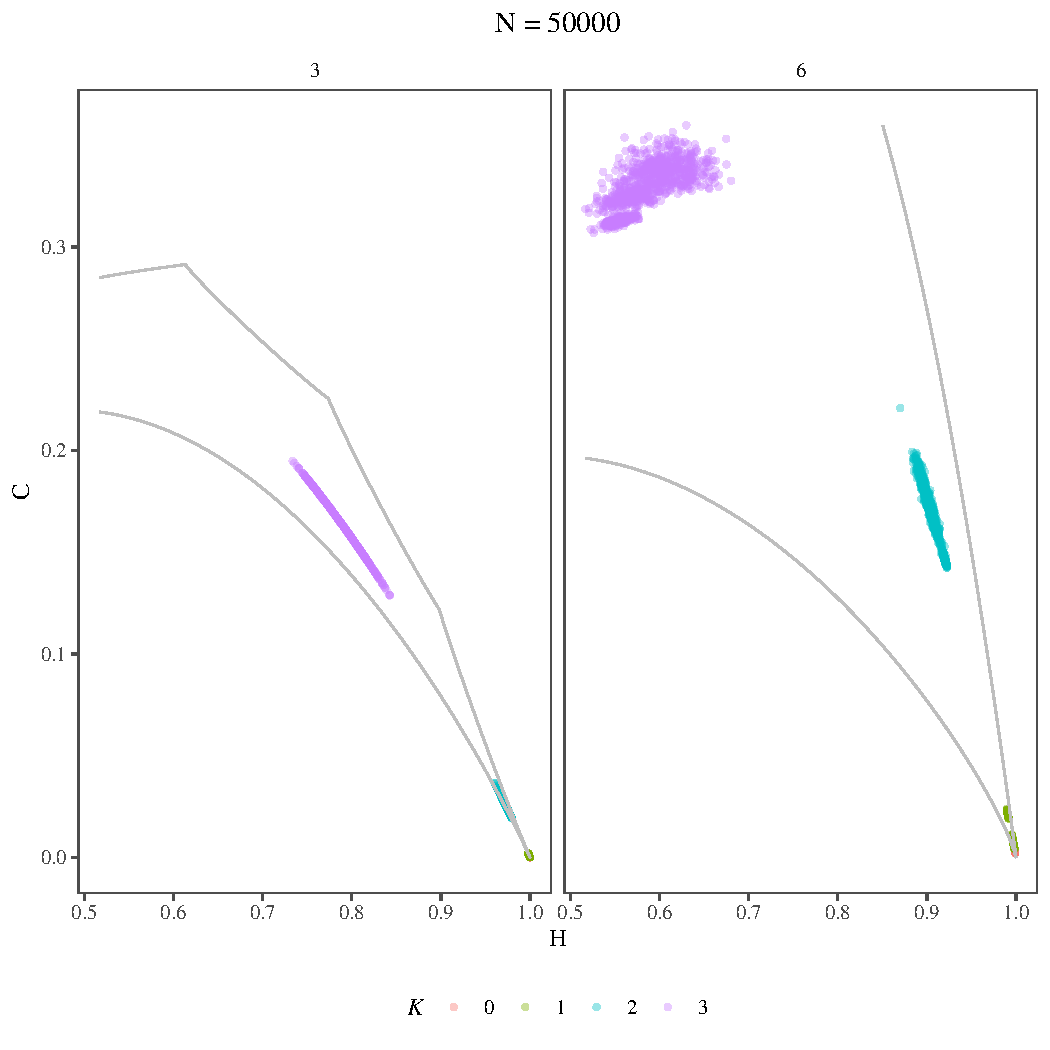
\includegraphics[width=\linewidth]{Figures/fk-descriptive-analysis.pdf}
    \caption{$f^{-k}$ noises in HC Plane}
    \label{fig:fk}
\end{figure}

\end{comment}

%\textcolor{red}{Justificar o tipo de an\'alise: regressão? bivariada clássica? não-paramétrica?}

%\textcolor{red}{Regi\~oes de confian\c ca}

\begin{comment}

\begin{figure}[H]
    \centering
    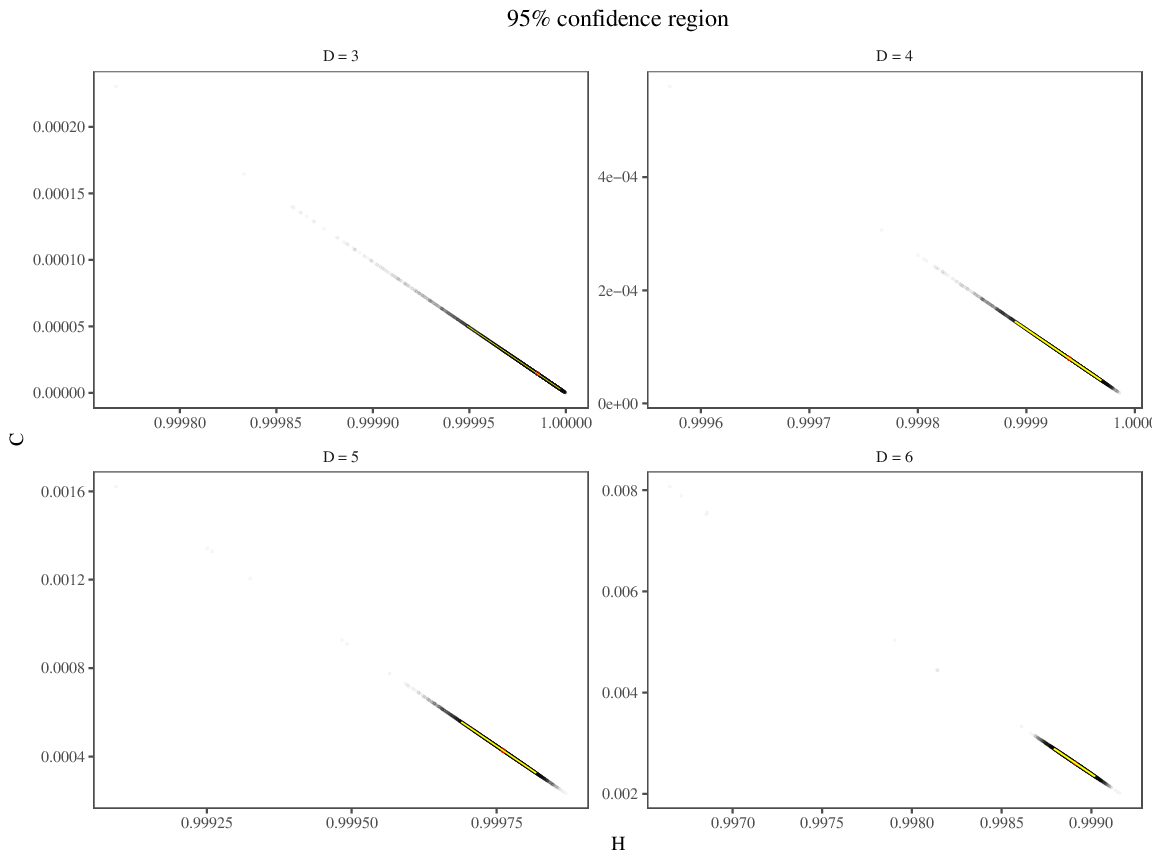
\includegraphics[width=\linewidth]{Figures/N50kBoxes95.png}
    \caption{}
    \label{fig:region95}
\end{figure}

\begin{figure}[H]
    \centering
    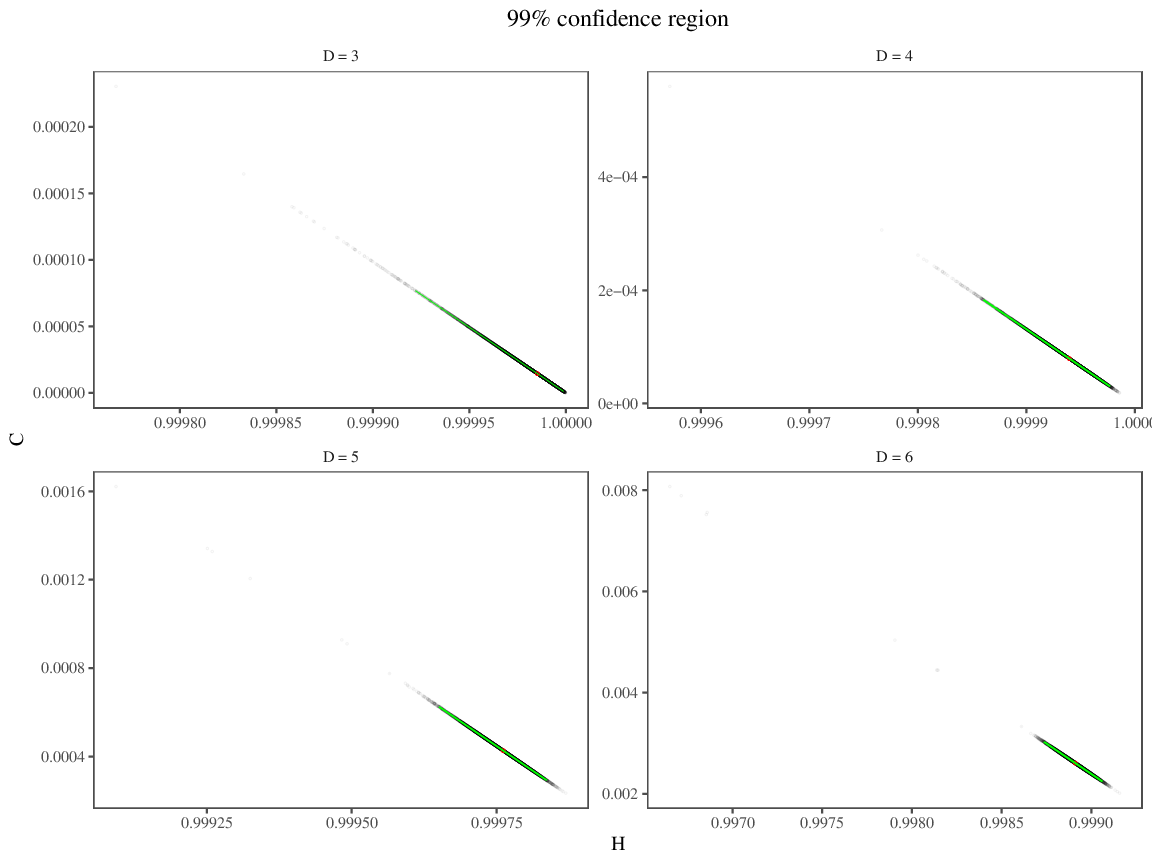
\includegraphics[width=\linewidth]{Figures/N50kBoxes99.png}
    \caption{}
    \label{fig:region99}
\end{figure}

\end{comment}


%\subsection{Analysis of the Empirical Confidence Regions}

\subsection{Analyzing of the Empirical Confidence Regions Injecting Correlation}
% k=0 white
% k=1 pink
% k=2 brown
% T = 1000, T = 5 10^5
% D= 3, D = 6

Fig.~\ref{fig:AllSystems} shows the behavior of random time series with different levels of correlation (by means of the $f^{-k}$ model) in the $(h,c)$ plane.
Knowing that such plane can discriminate between different system dynamics, several studies in the literature have used this approach in the investigation of methods of identification and characterization of randomness.
Although this same strategy can be used to characterize different levels of correlation structures, in our case, we want to analyze the impact of injecting such dynamics into noise under the aspect of confidence regions.

For carrying out the experiment, we used an ''emblematic'' time series as a basis.
This series consists of the sample corresponding to the median of the $(h,c)$ points used to build the confidence regions, thus expressing a representative sample of the dataset.
Fig.~\ref{fig:correlation}a. illustrates, respectively, the effect of a white noise time series when adding correlation structures related to the $f^{-k}$ series for $k \in \{0, 1, 2, 3 \}$.
As we can observe in the plane as the correlation between the observations increases, that is, $k > 0$, the randomness decreases and the entropy presented decreases, informing the loss of its stochastic characteristic.

Fig.~\ref{fig:correlation}b. illustrates the degree of limit correlation structure that can be added in white noise to eliminate it from the regions of confidence, where the red dot represents the original "emblematic" series.
When we have $k = 0$, the features of the sequence have a small variation, corroborating the premise that series of noise $f^{-k} = 0$ have a minimum correlation measure, not significantly changing the dynamics of the system.

\begin{figure}[H]
    \centering
	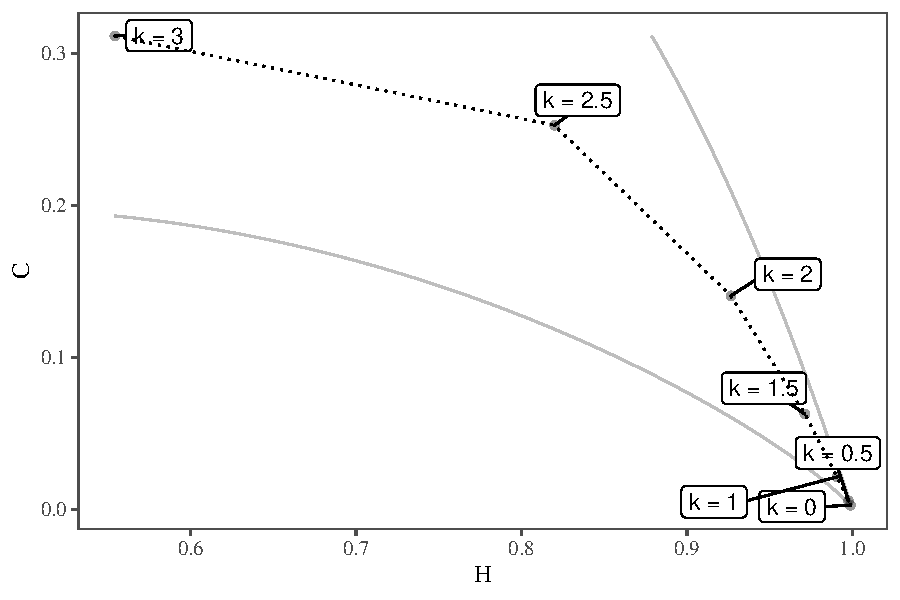
\includegraphics[width=.48\linewidth]{Figures/Correlation-Analysis-dotted.pdf}
    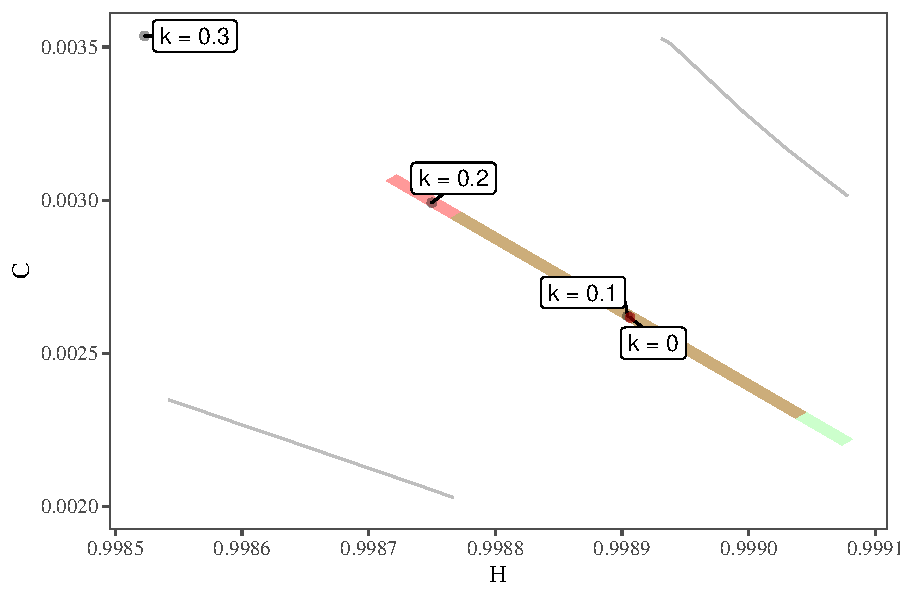
\includegraphics[width=.48\linewidth]{Figures/Correlation-Analysis-point.pdf}
    \caption{Correlation Structure Analysis
    }
    \label{fig:correlation}
\end{figure}
%In the following, we will present how the $(h,c)$ point of the ``emblematic'' sequence alters when injecting temporal correlation (by means of the $f^{-k}$ model).
%, and determinism (by a convex combination with a sine function).
%The $f^{-k}$: simulation

\begin{comment}
\subsection{Injecting Determinism}
Consider the emblematic sequence $\bm x=(x_1,\dots,x_N)$, which is mapped onto the point $(h,c)$.
In order to inject determinism in this sequence, we will analyze the effect of $\xi\in[0,1]$, by checking how the point $\big(h,c\big)(\xi)$ evolves in the $(H,C)$ plane, in which
\begin{equation}
\bm x'(j) = \xi \sin(10 \pi j/N) +(1-\xi) x_j.    
\label{Eq:DeterminismXi}
\end{equation}
With this, when $\xi=0$ we have the original sequence $\bm x$ and, thus, the original emblematic point $(h,c)$;
when $\xi=1$, we have pure determinism: five sine functions.
\end{comment}

\subsection{Revisiting the White Noise Hypothesis in the Literature}


\begin{table}[H]
	\centering
	\caption{Points inside the confidence regions}
	\label{tab:resultFinal}
	\begin{tabular}{c*{3}r}
		\toprule
		Algorithm & \multicolumn{1}{c}{$D$} & \multicolumn{1}{c}{\SI{95}{\percent}} & \multicolumn{1}{c}{\SI{99}{\percent}}\\
		\cmidrule(lr){1-1}
		\cmidrule(lr){2-2}
		\cmidrule(lr){3-3}
		\cmidrule(lr){4-4}
		Wichmann-Hill & 3 & 0.97 & 0.96\\ 
		Wichmann-Hill & 4 & 0.9675 & 0.9675\\ 
		Wichmann-Hill & 5 & 0.9725 & 0.965\\ 
		Wichmann-Hill & 6 & 0.97 & 0.97\\ 
		%\cmidrule(lr){1-4}
		%Marsaglia-Multicarry & 3 & 0.97 & 0.9625\\ 
		%Marsaglia-Multicarry & 4 & 0.97 & 0.9825\\ 
		%Marsaglia-Multicarry & 5 & 0.9625 & 0.9625\\ 
		%Marsaglia-Multicarry & 6 & 0.9675 & 0.9625\\ 
		\cmidrule(lr){1-4}
		Super-Duper & 3 & 0.9675 & 0.975\\ 
		Super-Duper & 4 & 0.9775 & 0.9725\\ 
		Super-Duper & 5 & 0.9675 & 0.985\\ 
		Super-Duper & 6 & 0.9825 & 0.965\\ 
		\cmidrule(lr){1-4}
		Knuth-TAOCP-2002 & 3 & 0.9775 & 0.9625\\ 
		Knuth-TAOCP-2002 & 4 & 0.965 & 0.98\\ 
		Knuth-TAOCP-2002 & 5 & 0.9625 & 0.9825\\ 
		Knuth-TAOCP-2002 & 6 & 0.9725 & 0.96\\  
		\cmidrule(lr){1-4}
		Knuth-TAOCP & 3 & 0.975 & 0.9775\\ 
		Knuth-TAOCP & 4 & 0.965 & 0.9725\\ 
		Knuth-TAOCP & 5 & 0.9875 & 0.985\\ 
		Knuth-TAOCP & 6 & 0.9725 & 0.975\\ 
		\cmidrule(lr){1-4}
		LEcuyer-CMRG & 3 & 0.98 & 0.98\\ 
		LEcuyer-CMRG & 4 & 0.9675 & 0.9725\\ 
		LEcuyer-CMRG & 5 & 0.965 & 0.9725\\ 
		LEcuyer-CMRG & 6 & 0.9625 & 0.97\\ 
		\cmidrule(lr){1-4}
		pcg64 & 3 & 0.97 & 0.9675\\ 
		pcg64 & 4 & 0.97 & 0.97\\ 
		pcg64 & 5 & 0.9775 & 0.9625\\ 
		pcg64 & 6 & 0.9575 & 0.9575\\ 
		\cmidrule(lr){1-4}
		Threefry & 3 & 0.9625 & 0.97\\ 
		Threefry & 4 & 0.975 & 0.97\\ 
		Threefry & 5 & 0.96 & 0.9625\\ 
		Threefry & 6 & 0.965 & 0.955\\ 
		\cmidrule(lr){1-4}
		Xoroshiro128+ & 3 & 0.975 & 0.9825\\ 
		Xoroshiro128+ & 4 & 0.995 & 0.9825\\ 
		Xoroshiro128+ & 5 & 0.98 & 0.9725\\ 
		Xoroshiro128+ & 6 & 0.9725 & 0.955\\ 
		\cmidrule(lr){1-4}
		MWC & 3 & 1 & 0.75\\
		MWC & 4 & 0.25 & 0.25\\ 
		MWC & 5 & 1 & 1\\ 
		MWC & 6 & 0 & 0\\ 
		\cmidrule(lr){1-4}
		MOT & 3 & 1 & 1\\ 
		MOT & 4 & 1 & 1\\ 
		MOT & 5 & 1 & 1\\ 
		MOT & 6 & 0.75 & 1\\ 
		\bottomrule 
	\end{tabular}
	\begin{tabular}{c*{3}r}
		\toprule
		Algorithm & \multicolumn{1}{c}{$D$} & \multicolumn{1}{c}{\SI{95}{\percent}} & \multicolumn{1}{c}{\SI{99}{\percent}}\\
		\cmidrule(lr){1-1}
		\cmidrule(lr){2-2}
		\cmidrule(lr){3-3}
		\cmidrule(lr){4-4}
		Xoshiro256+ (FOR) & 3 & 0.98 & 0.98\\ 
		Xoshiro256+ (FOR) & 4 & 0.9675 & 0.965\\ 
		Xoshiro256+ (FOR) & 5 & 0.9525 & 0.96\\ 
		Xoshiro256+ (FOR) & 6 & 0.9775 & 0.975\\
		\cmidrule(lr){1-4} 
		Mersenne-Twister & 3 & 0.9725 & 0.97\\ 
		Mersenne-Twister & 4 & 0.98 & 0.97\\ 
		Mersenne-Twister & 5 & 0.9725 & 0.9775\\ 
		Mersenne-Twister & 6 & 0.975 & 0.9725\\ 
		\cmidrule(lr){1-4}
		Randu & 3 & 0.2275 & 0.42\\ 
		Randu & 4 & 0 & 0\\ 
		Randu & 5 & 0 & 0\\ 
		Randu & 6 & 0 & 0\\ 
		\cmidrule(lr){1-4}
		LCG & 3 & 0.07 & 0.09\\ 
		LCG & 4 & 0 & 0\\ 
		LCG & 5 & 0 & 0\\ 
		LCG & 6 & 0 & 0\\ 
		\cmidrule(lr){1-4}
		LEH & 3 & 0.9825 & 0.98\\ 
		LEH & 4 & 0.9675 & 0.9775\\ 
		LEH & 5 & 0.9725 & 0.9775\\ 
		LEH & 6 & 0.9775 & 0.9825\\ 
		\cmidrule(lr){1-4}
		fBm & 3 & 0 & 0\\ 
		fBm & 4 & 0 & 0\\ 
		fBm & 5 & 0 & 0\\ 
		fBm & 6 & 0 & 0\\ 
		\cmidrule(lr){1-4}
		fGn & 3 & 0.9722 & 0.9874\\ 
		fGn & 4 & 0.9798 & 0.9773\\ 
		fGn & 5 & 0.9646 & 0.9773\\ 
		fGn & 6 & 0.9722 & 0.9545\\
		\cmidrule(lr){1-4}
		$f^{-k}$ & 3 & 0.9525 & 0.96\\ 
		$f^{-k}$ & 4 & 0.975 & 0.9725\\ 
		$f^{-k}$ & 5 & 0.98 & 0.9675\\ 
		$f^{-k}$ & 6 & 0.9775 & 0.975\\
		\cmidrule(lr){1-4}
		COM & 3 & 0.25 & 0.5\\ 
		COM & 4 & 0 & 0\\ 
		COM & 5 & 0 & 0\\ 
		COM & 6 & 0 & 0\\ 
		\cmidrule(lr){1-4}
		CCC & 3 & 0 & 0\\ 
		CCC & 4 & 0 & 0\\ 
		CCC & 5 & 0 & 0\\ 
		CCC & 6 & 0 & 0\\
		\bottomrule
	\end{tabular}
\end{table}



